\documentclass[a4paper,12pt]{article}
\usepackage{polyglossia}
\setmainlanguage{russian}
\usepackage{fontspec}
\setmainfont{Arial}
\setsansfont{Arial}
\setmonofont{Courier New}  % шрифт для листингов
% Явно указываем шрифт для кириллицы в моноширинном стиле
\newfontfamily{\cyrillicfonttt}{Courier New}

\usepackage{amsmath,amssymb,amsfonts}
\usepackage{geometry}
\usepackage{graphicx}
\usepackage{listings}
\usepackage{xcolor}

\geometry{top=2cm,bottom=2cm,left=3cm,right=1.5cm}

% Настройка стилей для отображения кода Python
\lstset{
    language=Python,
    basicstyle=\ttfamily\small,
    keywordstyle=\color{blue},
    stringstyle=\color{red},
    commentstyle=\color{green!60!black},
    numbers=left,
    numberstyle=\tiny\color{gray},
    stepnumber=1,
    numbersep=8pt,
    backgroundcolor=\color{gray!5},
    showstringspaces=false,
    breaklines=true
}

\begin{document}

% --- ТИТУЛЬНЫЙ ЛИСТ ---
\begin{titlepage}
    \centering
    \vspace*{1cm}
    \large ФГБОУ ВО КГТУ \\
    \large Кафедра высшей математики и информационных систем \\
    \vspace{4cm}
    \Large \textbf{ЛАБОРАТОРНАЯ РАБОТА № 1} \\
    \large По курсу: <<Методы оптимизации>> \\
    \large \textbf{Тема:} Необходимые и достаточные условия существования условного экстремума \\
    \vspace{1cm}
    \large \textbf{Вариант № 1.10} \\
    \vspace{4cm}
    \begin{flushright}
        \large \textit{Выполнил:} студент гр. ХХ-ХХ \\
        Иванов И. И. \\
        \vspace{0.5cm}
        \textit{Проверил:} преподаватель \\
        Петров П. П. \\
    \end{flushright}
    \vfill
    2026 г.
\end{titlepage}

\newpage

% --- ОТЧЕТ ---
\section{Цель работы}
1. Исследование необходимых и достаточных условий существования экстремума функции с учетом ограничений (условный экстремум).\\
2. Вычисление экстремумов функции.

\section{Постановка задачи}
Исследовать на условный локальный экстремум целевую функцию:
$$f(x) = (10\ln x_1 - 2)^2 + 10(x_2^2 + 2)^2 - 10 \rightarrow \text{extr}$$
при ограничениях типа неравенств:
$$\begin{cases}
    g_1(x) = x_1^2 + x_2^2 - 2 \le 0 \\
    g_2(x) = -x_1 \le 0 \\
    g_3(x) = -x_2 \le 0
\end{cases}$$
Область определения функции накладывает естественное условие $x_1 > 0$, откуда следует, что ограничение $g_2(x) \le 0$ строго пассивное.

\section{Аналитическое исследование}

\subsection{Необходимые условия первого порядка (Куна-Таккера)}
Составим классическую функцию Лагранжа ($\lambda_0=1$):
$$L(x, \lambda) = (10\ln x_1 - 2)^2 + 10(x_2^2 + 2)^2 - 10 + \lambda_1(x_1^2 + x_2^2 - 2) + \lambda_2(-x_1) + \lambda_3(-x_2)$$

Запишем систему уравнений стационарности:
$$\frac{\partial L}{\partial x_1} = \frac{20(10\ln x_1 - 2)}{x_1} + 2\lambda_1 x_1 - \lambda_2 = 0$$
$$\frac{\partial L}{\partial x_2} = 40x_2(x_2^2 + 2) + 2\lambda_1 x_2 - \lambda_3 = 0$$

Условия дополняющей нежесткости:
$$\lambda_1(x_1^2 + x_2^2 - 2) = 0, \quad \lambda_2(-x_1) = 0, \quad \lambda_3(-x_2) = 0$$
при $\lambda_j \ge 0$ для минимума.

\subsection{Поиск стационарных точек}
Так как $x_1 > 0$, то $\lambda_2 = 0$. Рассмотрим случай активного ограничения $g_3(x)$ ($x_2 = 0$) и пассивного $g_1(x)$ ($\lambda_1 = 0$).

Из уравнения по $x_2$: $40(0)(2) + 0 - \lambda_3 = 0 \implies \lambda_3 = 0$. \\
Из уравнения по $x_1$: $\frac{20(10\ln x_1 - 2)}{x_1} = 0 \implies 10\ln x_1 - 2 = 0 \implies x_1 = e^{0.2} \approx 1.221$.

Проверка допустимости $g_1(x^e)$: $(e^{0.2})^2 + 0^2 - 2 = e^{0.4} - 2 \approx -0.508 \le 0$ (выполняется).\\
Получена точка $x^e = (e^{0.2}, 0)$ при $\lambda^e = (0, 0, 0)^T$.

\subsection{Проверка достаточных условий второго порядка}
Вычислим матрицу вторых производных (Гессиан) функции Лагранжа в точке $x^e$:
$$\frac{\partial^2 L}{\partial x_1^2} = \frac{200}{x_1^2} - \frac{20(10\ln x_1 - 2)}{x_1^2} \Big|_{x^e} = \frac{200}{e^{0.4}} > 0$$
$$\frac{\partial^2 L}{\partial x_2^2} = 120x_2^2 + 80 + 2\lambda_1 \Big|_{x^e} = 80 > 0, \quad \frac{\partial^2 L}{\partial x_1 \partial x_2} = 0$$

Матрица $H = \begin{pmatrix} \frac{200}{e^{0.4}} & 0 \\ 0 & 80 \end{pmatrix}$ положительно определена. Второй дифференциал $d^2L > 0$ для любых ненулевых приращений, следовательно, $x^e$ — точка условного локального \textbf{минимума}.

Значение функции в точке экстремума:
$$f(x^e) = (2 - 2)^2 + 10(0 + 2)^2 - 10 = 30$$

\newpage
\section{Результаты программного моделирования}
Программная реализация выполнена на языке Python. Численное решение полностью совпало с теоретическим.

\begin{figure}[h!]
    \centering
    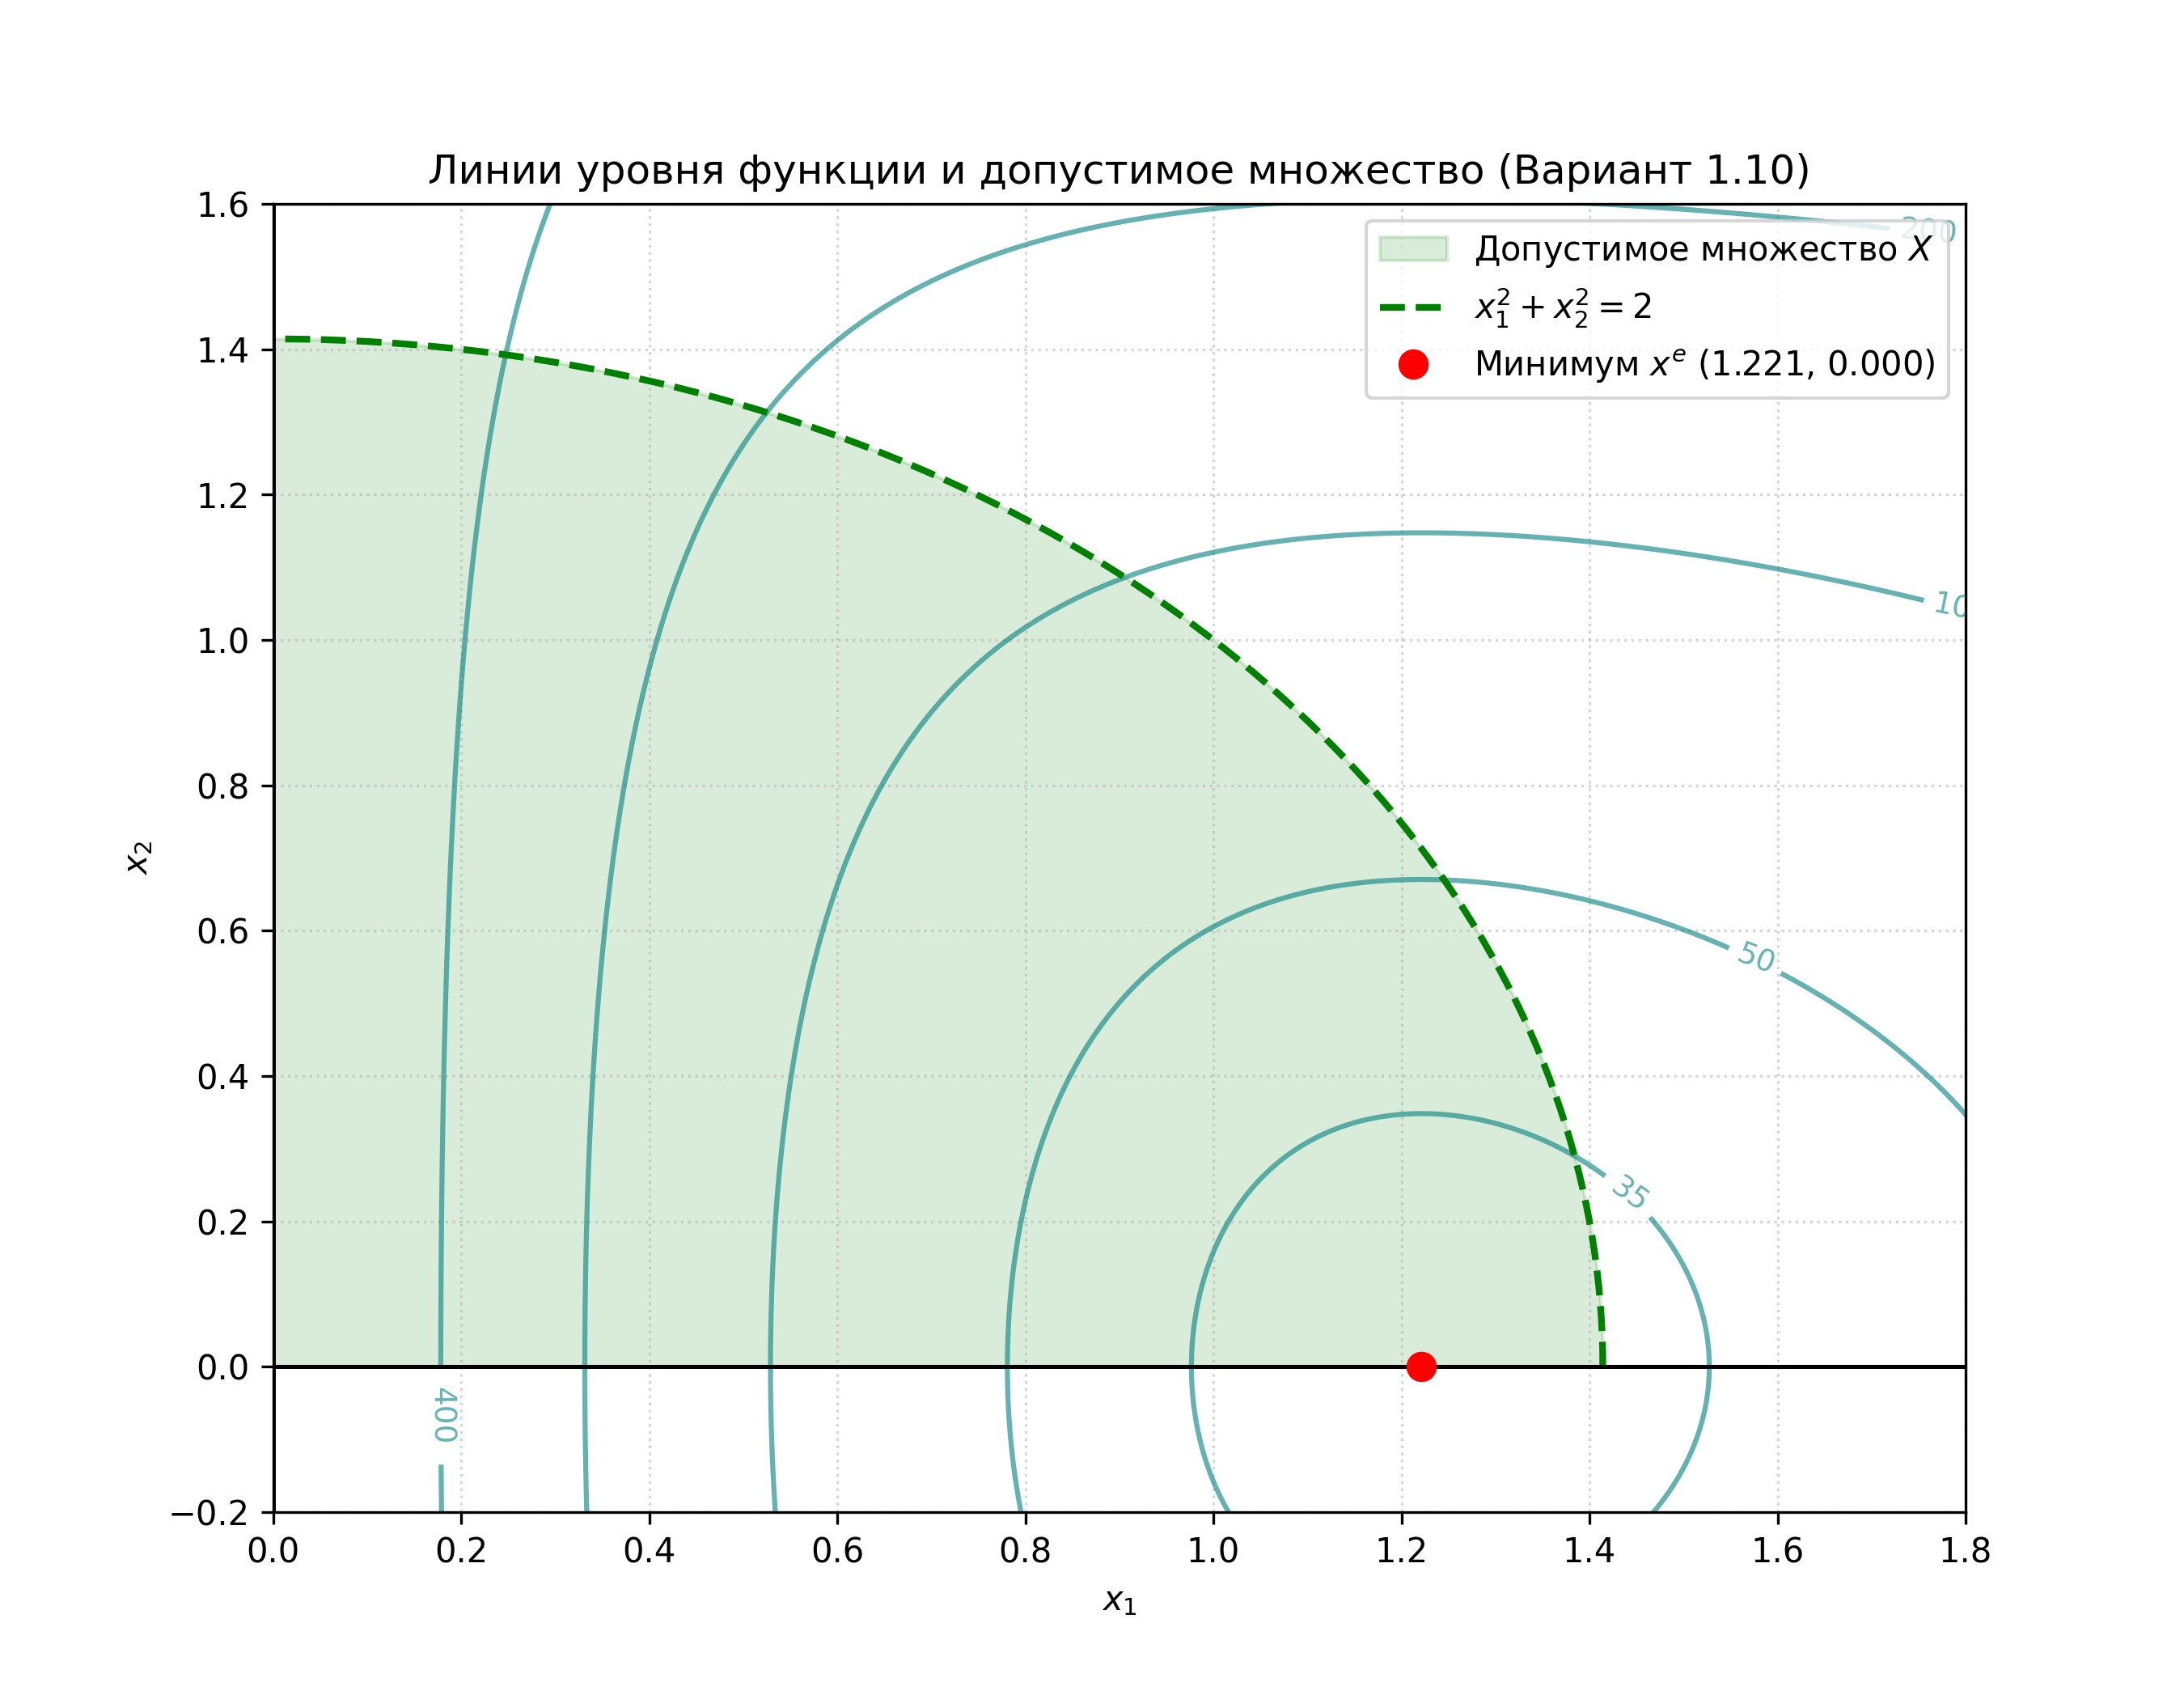
\includegraphics[width=0.75\textwidth]{plot_opt.png}
    \caption{Линии уровня функции и допустимое множество}
    \label{fig:plot}
\end{figure}

\section{Исходный код программы}
\begin{lstlisting}
# Вставь сюда код скрипта из шага 1
\end{lstlisting}

\begin{thebibliography}{1}
\bibitem{lab} Методические указания к лабораторной работе №1 <<Необходимые и достаточные условия существования условного экстремума>>.
\end{thebibliography}

\end{document}